\documentclass{article}
\addtolength{\textheight}{3.5cm}
\addtolength{\topmargin}{-1.5cm}
\addtolength{\textwidth}{4cm}
\addtolength{\oddsidemargin}{-2cm}
\addtolength{\evensidemargin}{-2cm}

\usepackage{graphicx,amsmath,amssymb,txfonts}
\usepackage{ascmac,color,url}


\usepackage[yyyymmdd,hhmmss]{datetime}

\title{Report of an experiment using Keras}
\author{Yoshihiro Mizoguchi}
\date{\today \currenttime}

\begin{document}
\maketitle

We made several trials using Keras to observe machine learnig
effects using Keras.
We consider neural networks which consider a board score
of the domineering game.
The domineering games with small size are well considered
and we can compute all game records within practical time.
But to investigage a convergence phenomena of machine learnig
statuses, we choose this game using $4 \times 4$ board as an example.

At first, we compute the number of status of boards in the game.
The number of possible statuses are 2442.
Since we can identify symmetric boards and rotated boards are same.
So the essential number of possible statuses are 488.
Further, this game is profitable for the 1st player.
There are 4 possible positions for the 1st player's 1st positions
identifing syumetric statuses.
If the 1st player choose the 2 of them, then he is determined to win
if he choose appropriate positions for each his turn.
If he missed to choose the first 2 profittable positions,
the 2nd player is determined to win.

We note that the 1st player should choose a one of 
the following two reduced statuses.
\begin{center}
\begin{tabular}{c}
\begin{tabular}{|c|c|c|c|}\hline
.&.&.&.\\ \hline
.&.&.&O\\ \hline
.&.&.&O\\ \hline
.&.&.&.\\ \hline
\end{tabular} \\
{\tiny 6,24576}
\end{tabular}
\begin{tabular}{c}
\begin{tabular}{|c|c|c|c|}\hline
.&.&.&.\\ \hline
.&.&O&.\\ \hline
.&.&O&.\\ \hline
.&.&.&.\\ \hline
\end{tabular} \\
{\tiny 96,1536}
\end{tabular}
\end{center}
If the 1st player chooses a one of 
the following two reduced statuses,
the 2nd player is determined to win.
\begin{center}
\begin{tabular}{c}
\begin{tabular}{|c|c|c|c|}\hline
.&.&.&.\\ \hline
.&.&.&.\\ \hline
.&.&.&O\\ \hline
.&.&.&O\\ \hline
\end{tabular} \\
{\tiny 3,12,12288,49152}
\end{tabular}
\begin{tabular}{c}
\begin{tabular}{|c|c|c|c|}\hline
.&.&.&.\\ \hline
.&.&.&.\\ \hline
.&.&O&.\\ \hline
.&.&O&.\\ \hline
\end{tabular} \\
{\tiny 48,192,768,3072}
\end{tabular}
\end{center}
Although this game is determined at the first stage, it is a good
example to investigation of machine learning options and statuses
at the begining.

\section{Dense Neural Network}

\begin{figure}
\begin{center}
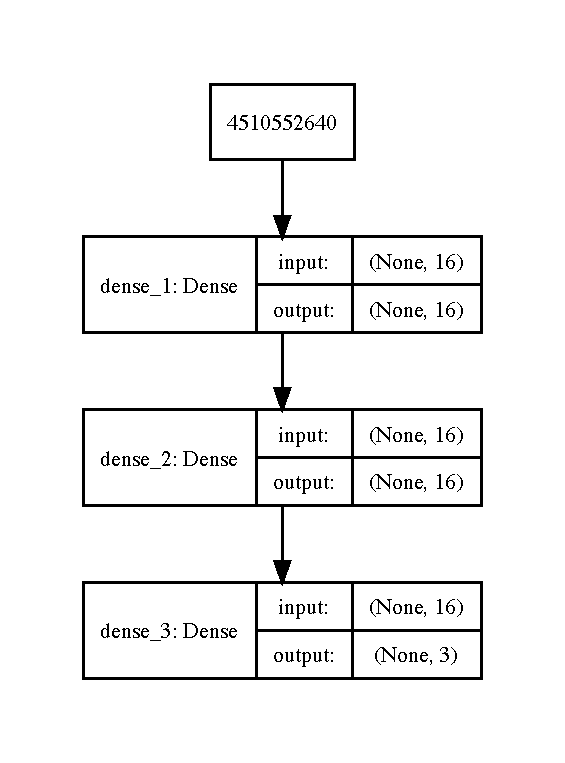
\includegraphics[width=6cm]{../dump/model1.pdf}
\end{center}
\begin{verbatim}
#
# Keras implementation
#
model = Sequential()
model.add(Dense(16, activation='relu', input_dim=16))
model.add(Dense(16, activation='tanh'))
model.add(Dense(3, activation='softmax'))
model.compile(loss='categorical_crossentropy',
              optimizer='sgd', metrics=['accuracy'])
\end{verbatim}
\caption{Simple Dense Nueral Network}\label{fig:1}
\end{figure}

At first, we started to choose a simple dense network(cf. Fig.\ref{fig:1}).
We consider a score function of a board status.
Each board with dominos have an advantage for a player,
we decide a score of the board to 1 if the next player fails.
That is a player can check his action's evaluation
by doing an act and evaluating the score of the board.

This is a simple network, we put all possible 2442 cases 
board scores as a training data.

We showed the learning records of 1000 epochs traing
and 9000 epochs traing.

\begin{figure}
\begin{center}
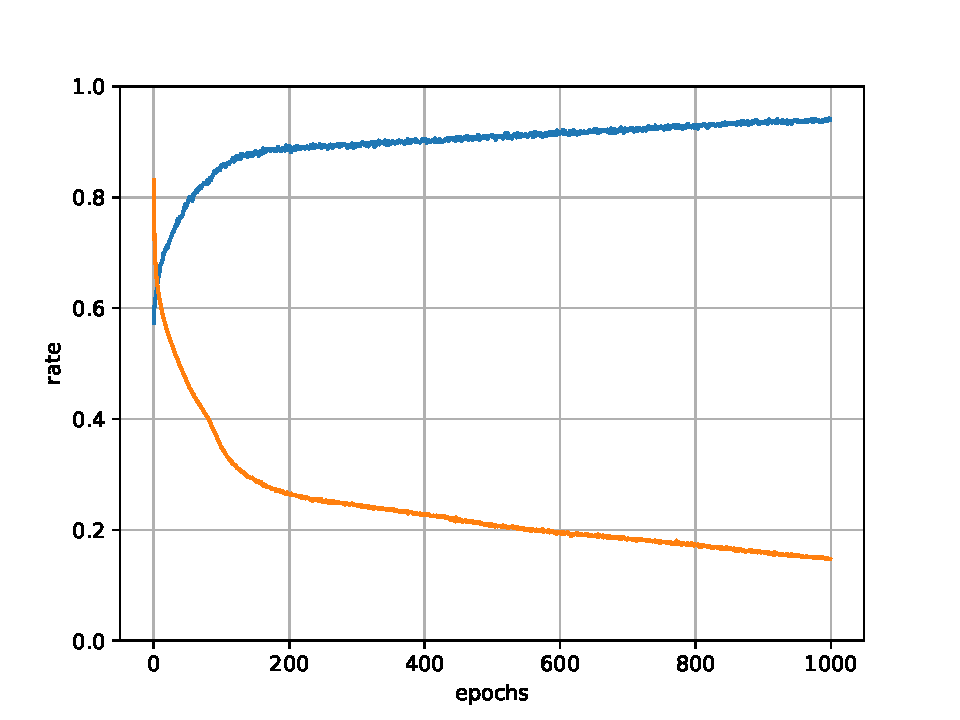
\includegraphics[width=6cm]{../dump/model1_01000.pdf}
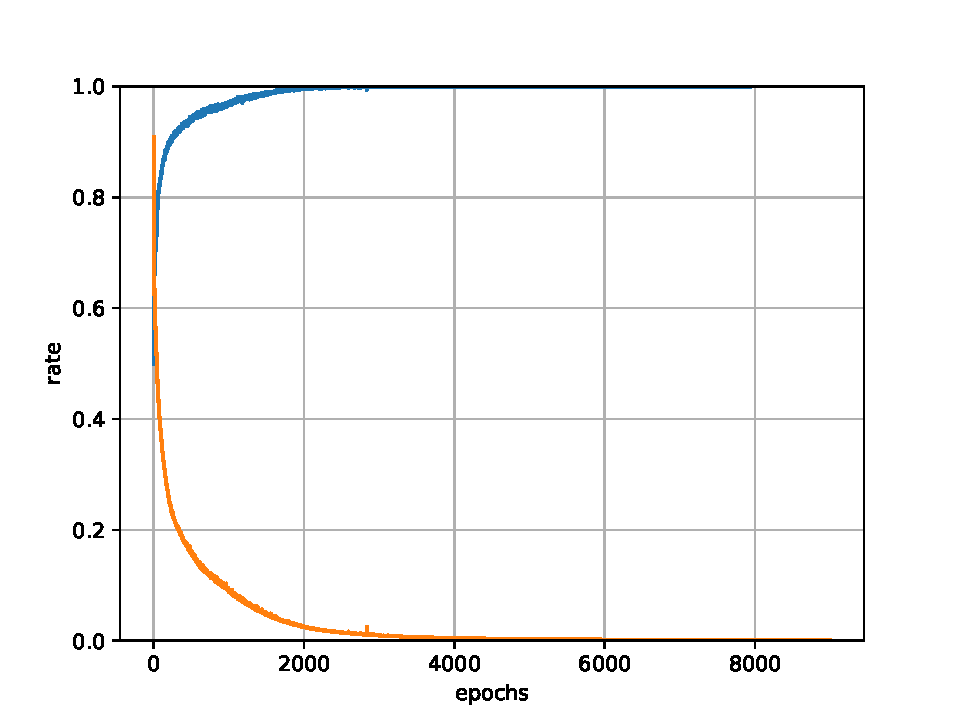
\includegraphics[width=6cm]{../dump/model1_09000.pdf}
\end{center}
\caption{Simple Dense Nueral Network Training}\label{fig:2}
\end{figure}

\section{Convolutional Neural Network}

\begin{figure}
\begin{center}
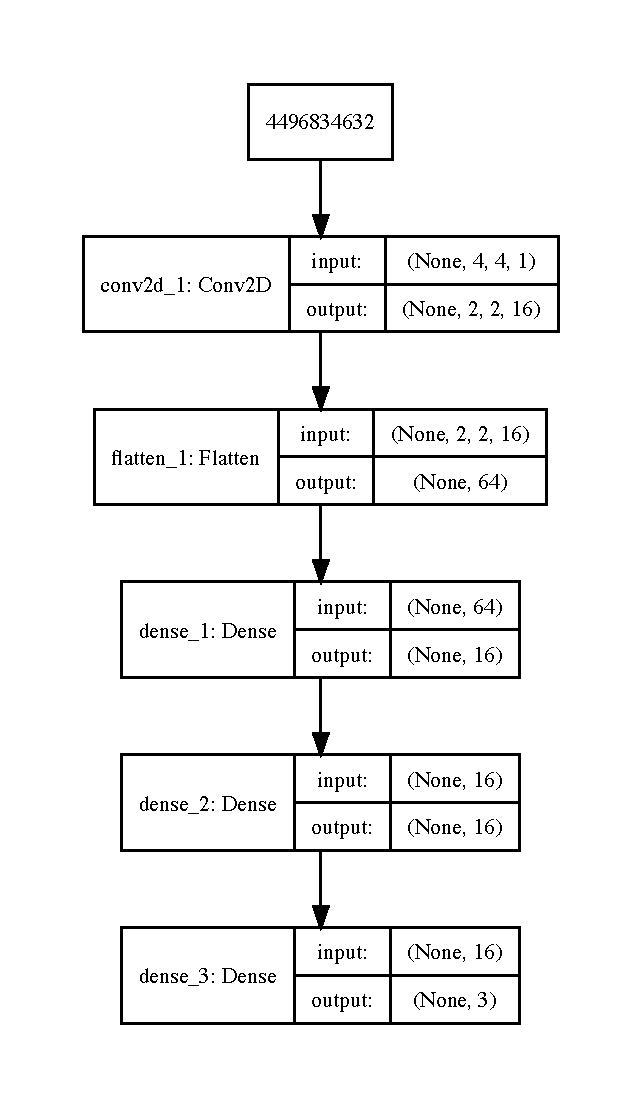
\includegraphics[width=6cm]{../dump/model2.pdf}
\end{center}
\begin{verbatim}
#
# Keras implementation
#
model = Sequential()
model.add(Conv2D(16, kernel_size=(3, 3),
                 activation='relu',input_shape=(4,4,1)))
model.add(Flatten())
model.add(Dense(16, activation='relu'))
model.add(Dense(16, activation='tanh'))
model.add(Dense(3, activation='softmax'))
model.compile(loss='categorical_crossentropy',
              optimizer='sgd', metrics=['accuracy'])
\end{verbatim}
\caption{Simple Convolutional Nueral Network}\label{fig:3}
\end{figure}

Next, we introduce a simple convolutional network(cf. Fig.\ref{fig:3}).

We showed the learning records of 1000 epochs traing
and 2000 epochs traing.
As you can see, it is easy to understand advantages
of convolution layers.

\begin{figure}
\begin{center}
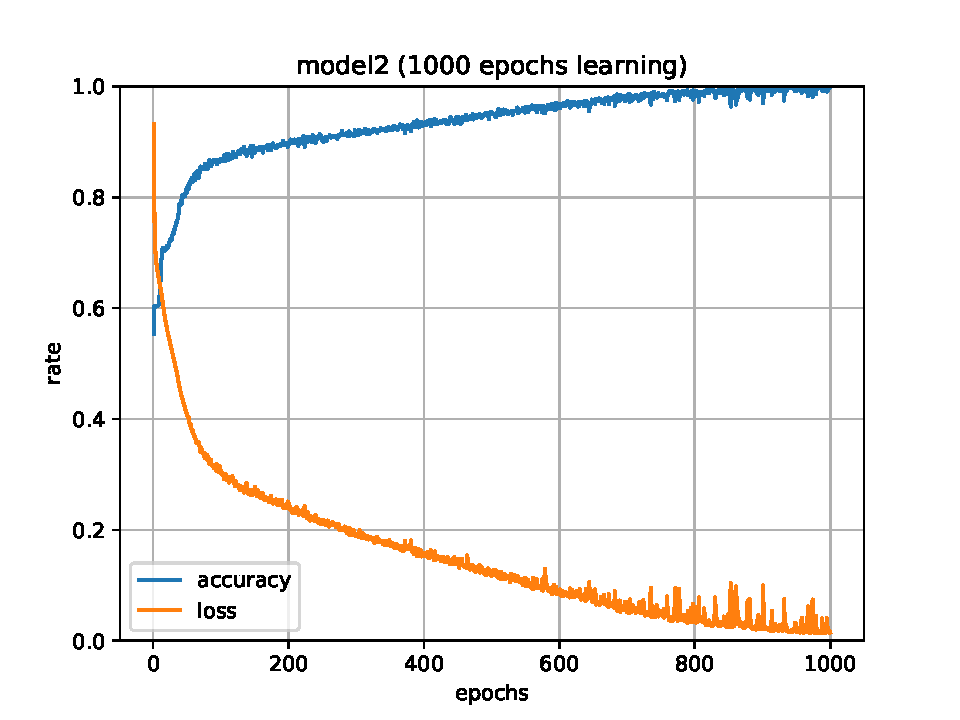
\includegraphics[width=6cm]{../dump/model2_01000.pdf}
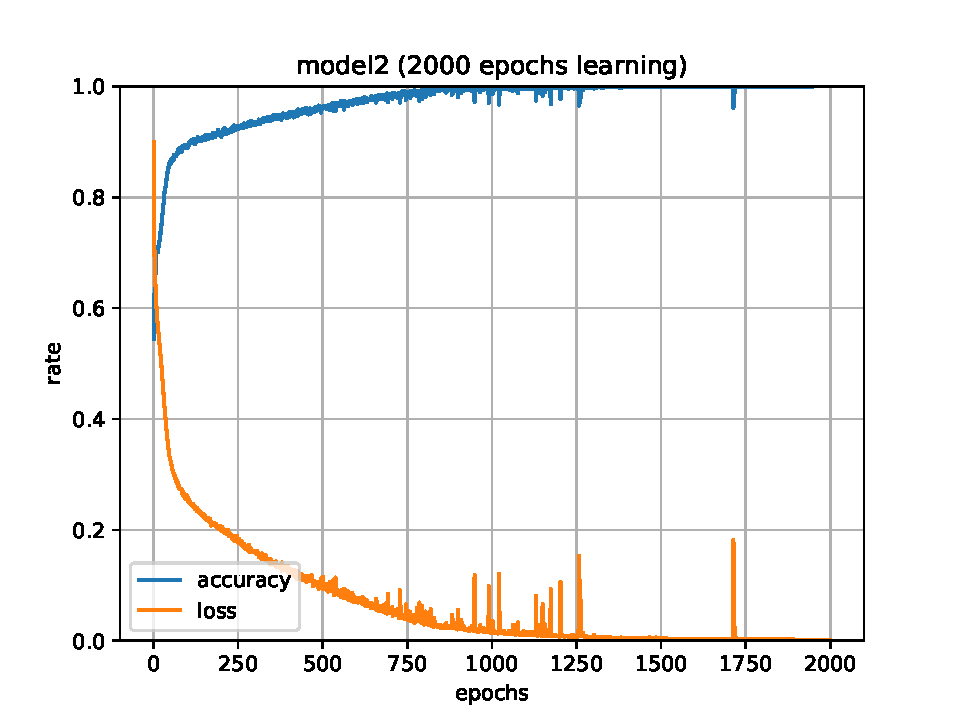
\includegraphics[width=6cm]{../dump/model2_02000.pdf}
\end{center}
\caption{Simple Convolutional Nueral Network Training}\label{fig:4}
\end{figure}

\section{AI Players for domineering game}
After learning, we can make an AI player using our learned neural network.

\begin{verbatim}
 class AIPlayer:
    def __init__(self, modelname='model1', epochs=10):
        self.modelname = modelname
        self.epochs = epochs
        fn = './'+modelname+"_{0:05d}".format(epochs)
        self.model = load_model(fn+'.h5')
        return None
    def tolist(self):
        for x in self.perfect:
            y=[x[0]]+(x[1].reshape((16)).tolist())
        return y
    def eval(self, board):
        b = board.reshape((16)).tolist()
        r = self.model.predict(np.array([b]))
        return([0,1,-1][np.argmax(r)])
    def play(self, board):
        acts = calc_actions(board)
        a = []
        for action in acts:
            next_state = calc_next_state(board,action)
            v = self.eval(next_state)
            if (v == 1):
                a.append(action)
        if (a == []):
            return choice(acts)
        else:
            return choice(a)
\end{verbatim}

\end{document}
